\documentclass[letterpaper,12pt]{article}
\usepackage[utf8]{inputenc}
\usepackage{fullpage}
\usepackage{courier}
\usepackage[margin=0.75in]{geometry}
\usepackage{listings}
\usepackage{color}
\usepackage{graphicx}
\usepackage[width=5in]{caption}
\usepackage{hyphenat}

% Format a sectionless paragraph
\newcommand*\unparagraph{
	\par
	\nopagebreak
	\vskip3.25ex plus1ex minus.2ex
	\noindent
}

% define extra colors
\definecolor{dkgreen}{rgb}{0,0.6,0}
\definecolor{purple}{RGB}{159,0,197}

% define the code listing format
\lstset{
	language=C++,
	basicstyle=\footnotesize\ttfamily,
	backgroundcolor=\color{white},
	showspaces=false,
	showstringspaces=false,
	frame=none,
	tabsize=3,
	keywordstyle=\color{purple},
	commentstyle=\color{dkgreen},
	stringstyle=\color{blue},
	escapeinside={\%*}{*)}
}

% efine the title/header
\title{\Large CS 3468\\Lab 1} 
\author{Jared Wallace}
\date{}

\begin{document}

\maketitle

\vspace{30mm}

\section*{Introduction to Embedded Systems Programming}
Today we are going to cover the overall workflow of the labs
we will be completing, as well as gaining familiarity with the
equipment we will be using.

\section*{Objectives}
\begin{enumerate}
	\item Understand the sensor development environment
	\item Learn to compile and install sensor applications
	\item Understand the functionality of an embedded system
\end{enumerate}

\section*{Tasks}
\begin{enumerate}
   \item Inspect the sensor development kit
      \begin{itemize}
          \item The development kit includes two Micaz \textbf{motes}, one MDA100 \textbf{sensor},
            one MIB520 \textbf{programming board}, one USB cable, and several batteries.
               The development software has already been installed on the lab computer.
               \textit{This is a typical development kit for any embedded system.}
            \item The \textbf{mote} is the actual embedded system that communicates with
               other motes and runs various kinds of embedded applications. The
               sensor measures temperature and light intensity of the environment
               and transmits the sensing data to the attached mote.
               The mote then processes or sends the data to other motes.
         \item The programming board is responsible for loading executable application
               images onto the mote and for configuring the mote. The programming board
               also provides interfaces for debugging sensor applications and
               gathering data from the mote.
         \item The USB cable connects the programming board with the computer.
               Sensor applications developed in the computer are transferred
               to the mote via the USB cable, through the programming board. The
               reverse is also true, the mote can output data to the computer,
               through the programming board and the USB cable.
         \item Now unplug the sensor from the mote. If you inspect the
               sensor board, you can see the actual sensors for light and temperature.
               \textbf{Note:} The sensor can only acquire data, it cannot communicate with
               other sensors or process sensing data by itself.
         \item The mote has one antenna, one embedded processor, and one slot.
               The antenna is for communicating with other motes. The slot is
               the interface for plugging in either the sensor or the programming board.
               If the sensor is plugged into the slot, the mote can obtain data from the
               sensor. If the programming board is plugged into the slot, the mote can
               obtain the application image from the computer and use it to program the on-board
               embedded processor. The programmable embedded processor is the central
               processing unit. It runs sensor applications and controls all peripherals
               of the sensor.
         \item Now, please remove the batteries, if any, from the mote, firmly plug the programming
               board into the mote, and use the USB cable to connect the programming board
               to the computer. We are now ready to compile and run our first sensor application.
         \item \emph{\textbf{Always remove any batteries when plugging the programming board into the mote!!}}
      \end{itemize}
   \item Compile and install the sensor application \textbf{Blink}
      \begin{enumerate}
         \item Open a terminal, and type the following command:
               \begin{lstlisting}
               mkdir Embedded
               mkdir Embedded/lab1
               \end{lstlisting}
               This will create a directory to store your lab files. Place the lab files from the website
               into the folder "lab1" that you created.
         \item Type 
               \begin{lstlisting}
               cd Embedded/lab1
               make micaz
               \end{lstlisting}
               to compile and link the Blink application. You will then see some messages in
               the terminal showing the progress of compilation and linking.
         \item Now, you can see that a new folder “build/micaz” has been created, in
               which you will find the executable application images “main.srec” and “main.ihex”.
               However, keep in mind that the image is not executable in the computer.
               It is only executable in the mote.
         \item Now, connect the USB cable to the computer and the programming board.
         \item Now you can type
               \begin{lstlisting}
               sudo make micaz install mib510,/dev/ttyUSB0
               \end{lstlisting}
               to install the Blink application in the mote. (You must be root to install to the hardware). The password is "Embedded". You will see some messages showing that the executable image
               is being transferred into the mote.
         \item At this point, you should see LEDs blinking on the mote. Unplug the programming board
               from the mote and insert the two batteries. Make sure you turn the switch on the mote to the
               "on" position. You should see more LED's blinking.
      \end{enumerate}
\end{enumerate}

\section*{Lab Report Instructions}
No report is required for this lab.

% Comic at the bottom
\begin{figure}[ht!]
	\centering
	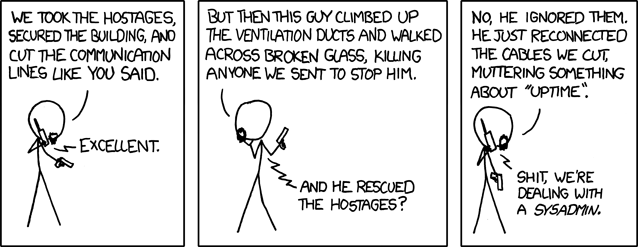
\includegraphics[width=5in]{devotion_to_duty.png}
	\caption*{The weird sense of duty really good sysadmins have can border on the sociopathic, 
		but it's nice to know that it stands between the forces of darkness and your cat blog's servers.}
\end{figure}
\end{document}
